\providecommand{\main}{../../../..}
\documentclass[\main/dresen_thesis.tex]{subfiles}

\begin{document}
  As the studied solvent/co-solvent dispersions are composed of a fast and slow evaporating components, the drop casting process subdivides into two parts.
  The first, where the primary solvent of the dispersion evaporates and the second where the slowly evaporating secondary phase is gently removed.

  \subsubsection{First Stage: Fast Evaporating Component}
    \begin{figure}[tb]
      \centering
      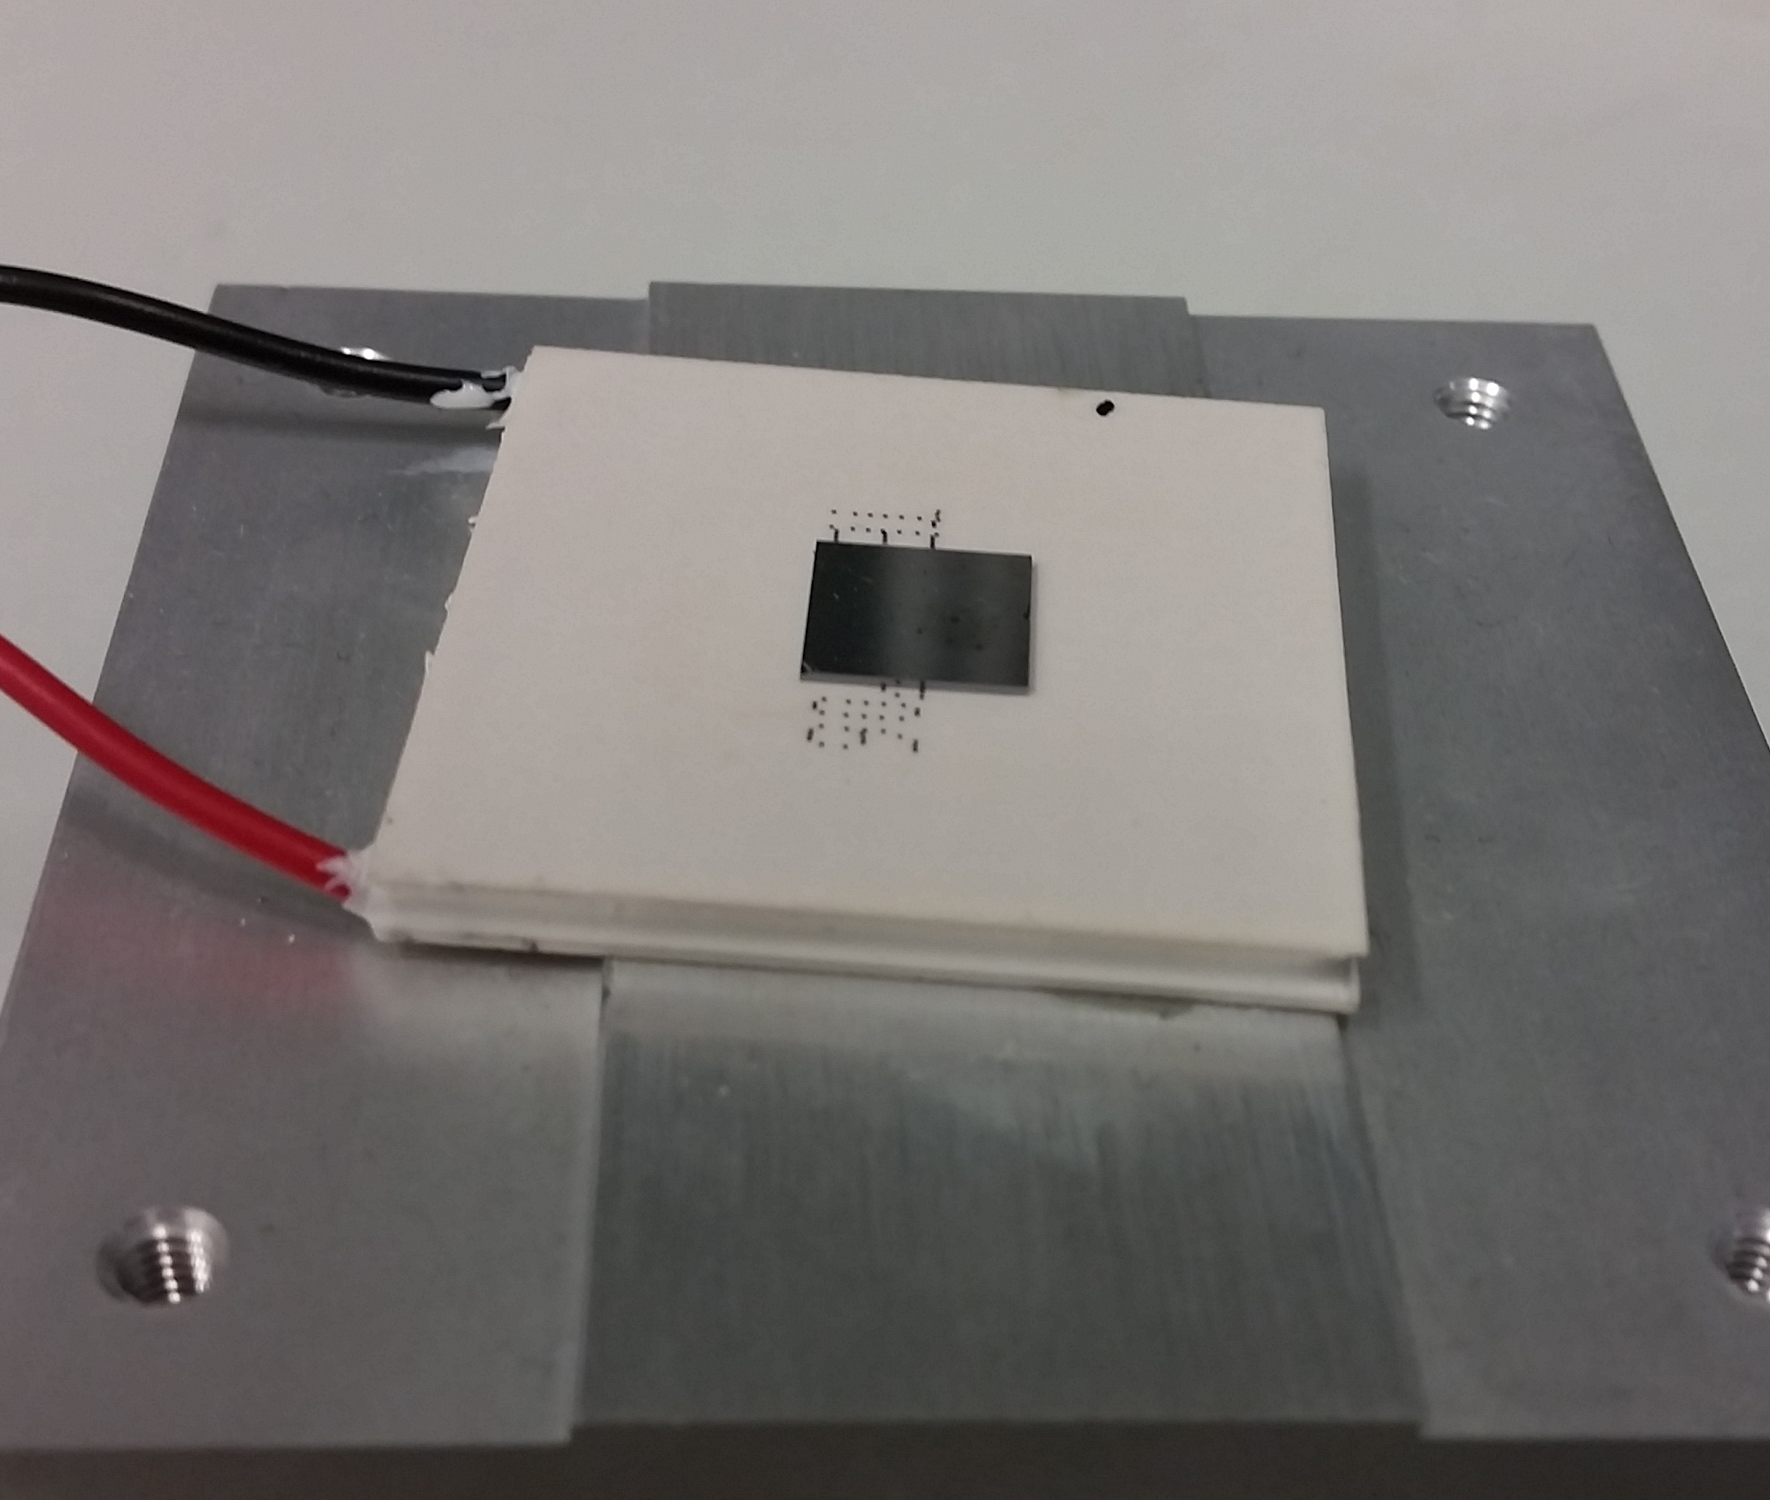
\includegraphics{monolayers_preparation_heating_stage}
      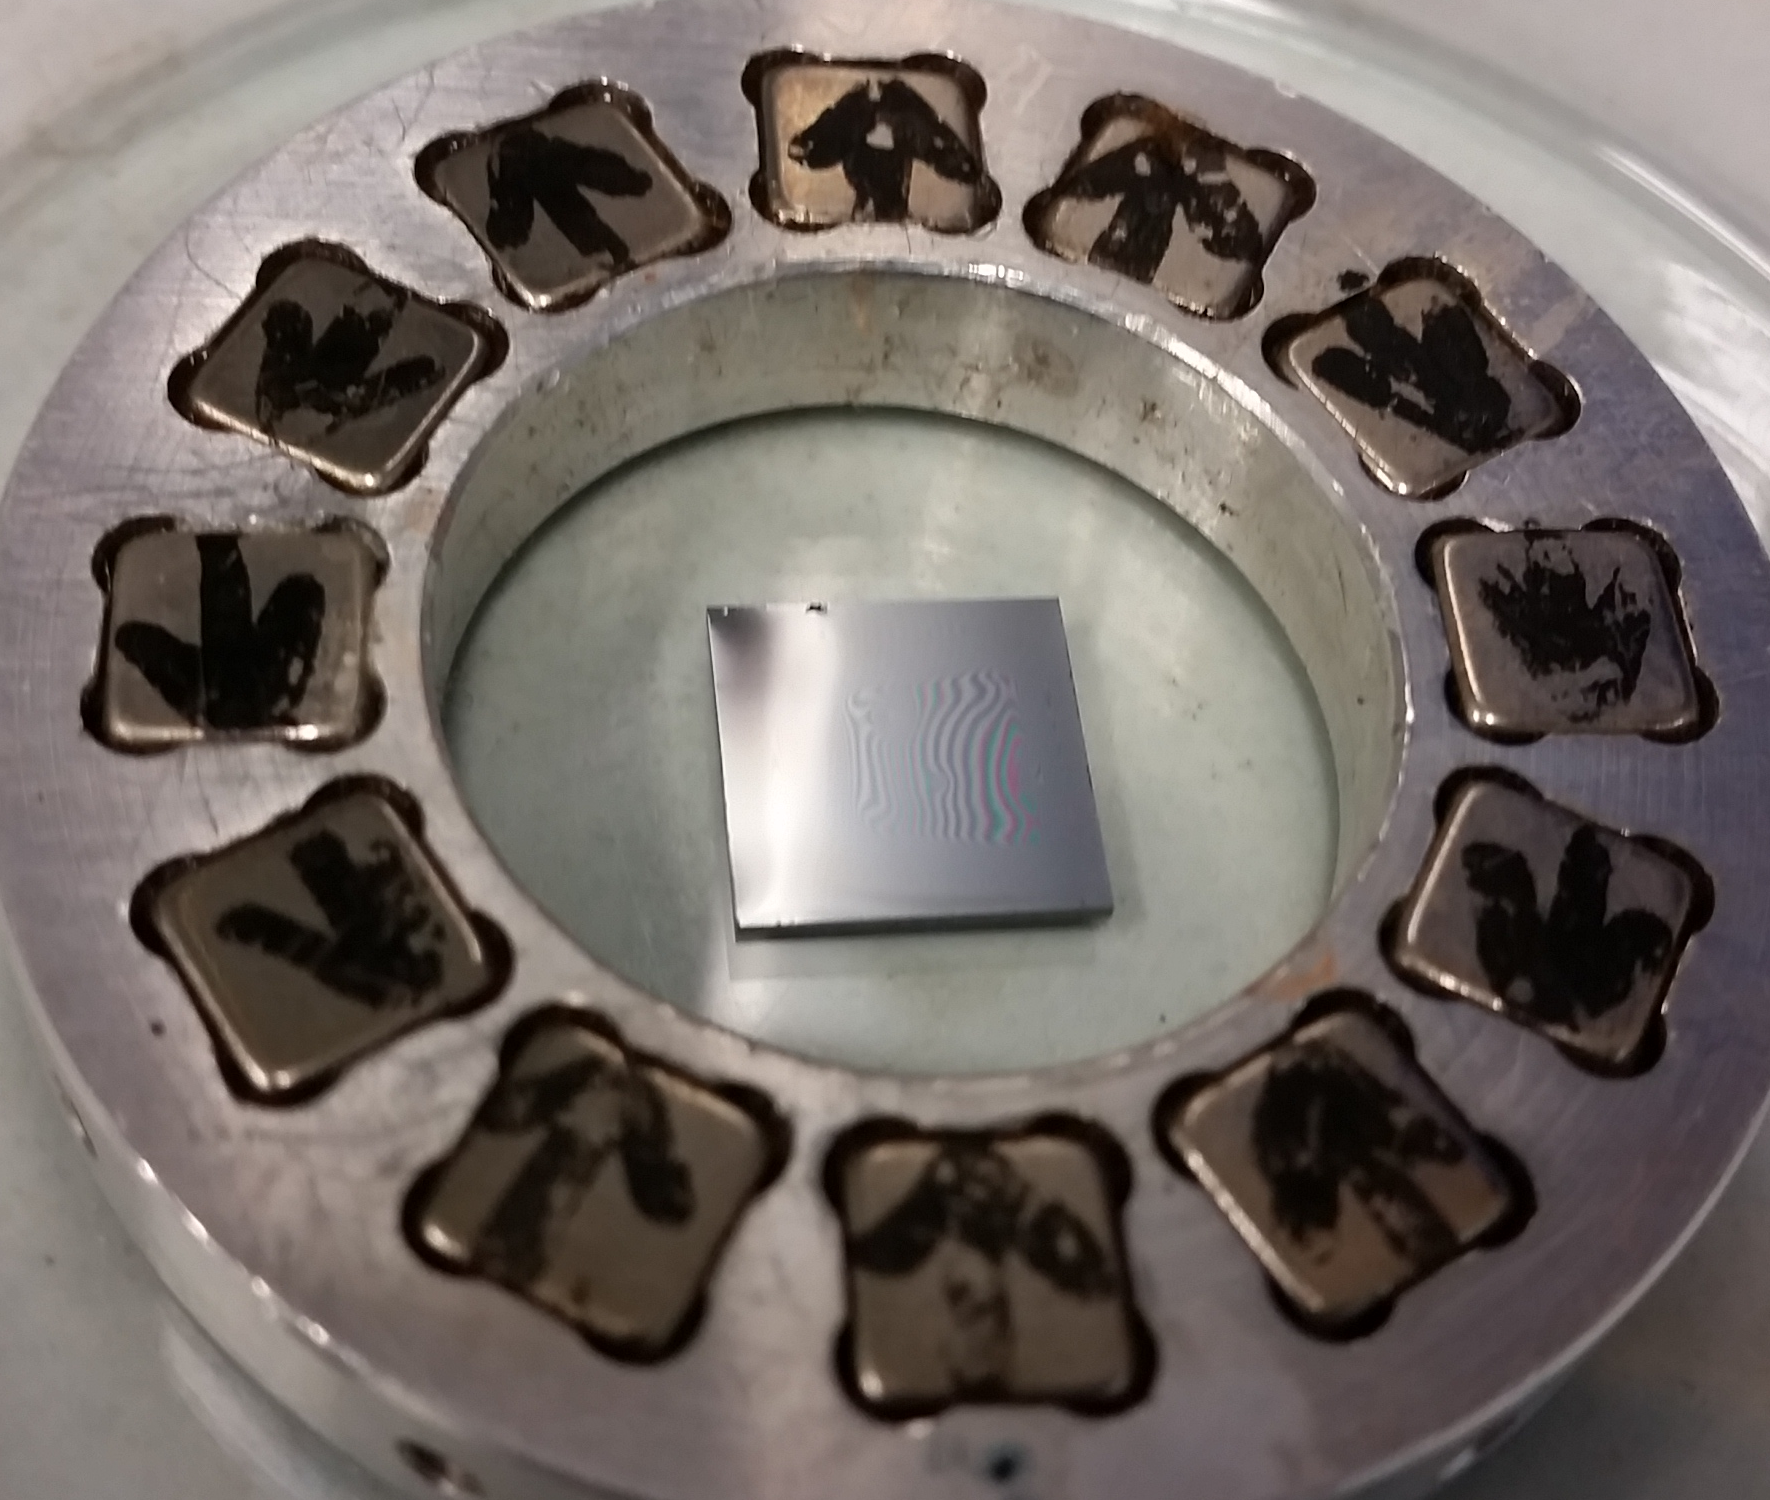
\includegraphics{monolayers_preparation_magnetic_field}
      \caption{\label{fig:monolayers:preparation:dryingConditions:varyConditions}The drying conditions for the droplet on the substrate can be varied continuously in temperature by means of a Peltier element (left) or an in-plane magnetic field can be added by using a Halbach cylinder (right).}
    \end{figure}
    It was attempted to slow down the first stage of evaporation for the drop casting process, by enriching the solvent atmosphere of the container, which is achieved by closing the containers by a glass lid and adding additional pieces of cloth that are soaked in solvent into the petri dish. % DD90
    However, direct comparison of the obtained structures showed no qualitative change in the long range order and therefore the simplest procedure in an open container was favored.

    The surface temperature of the substrate was varied by using a Peltier element as shown in the left image of \reffig{fig:monolayers:preparation:dryingConditions:varyConditions}. %DD169
    It became visible that once the primary solvent is evaporated, and the wafer surface is cooled with a minimal applied voltage to the Peltier element, the 1-octadecene quickly freezes at substrate temperatures around $16 \unit{^\circ C}$.
    The resulting layers show an even coverage of the wafer, but no long range order in between the nanoparticles, and therefore the Peltier element is considered as not helpful for the drying process.

    \begin{figure}[tb]
      \centering
      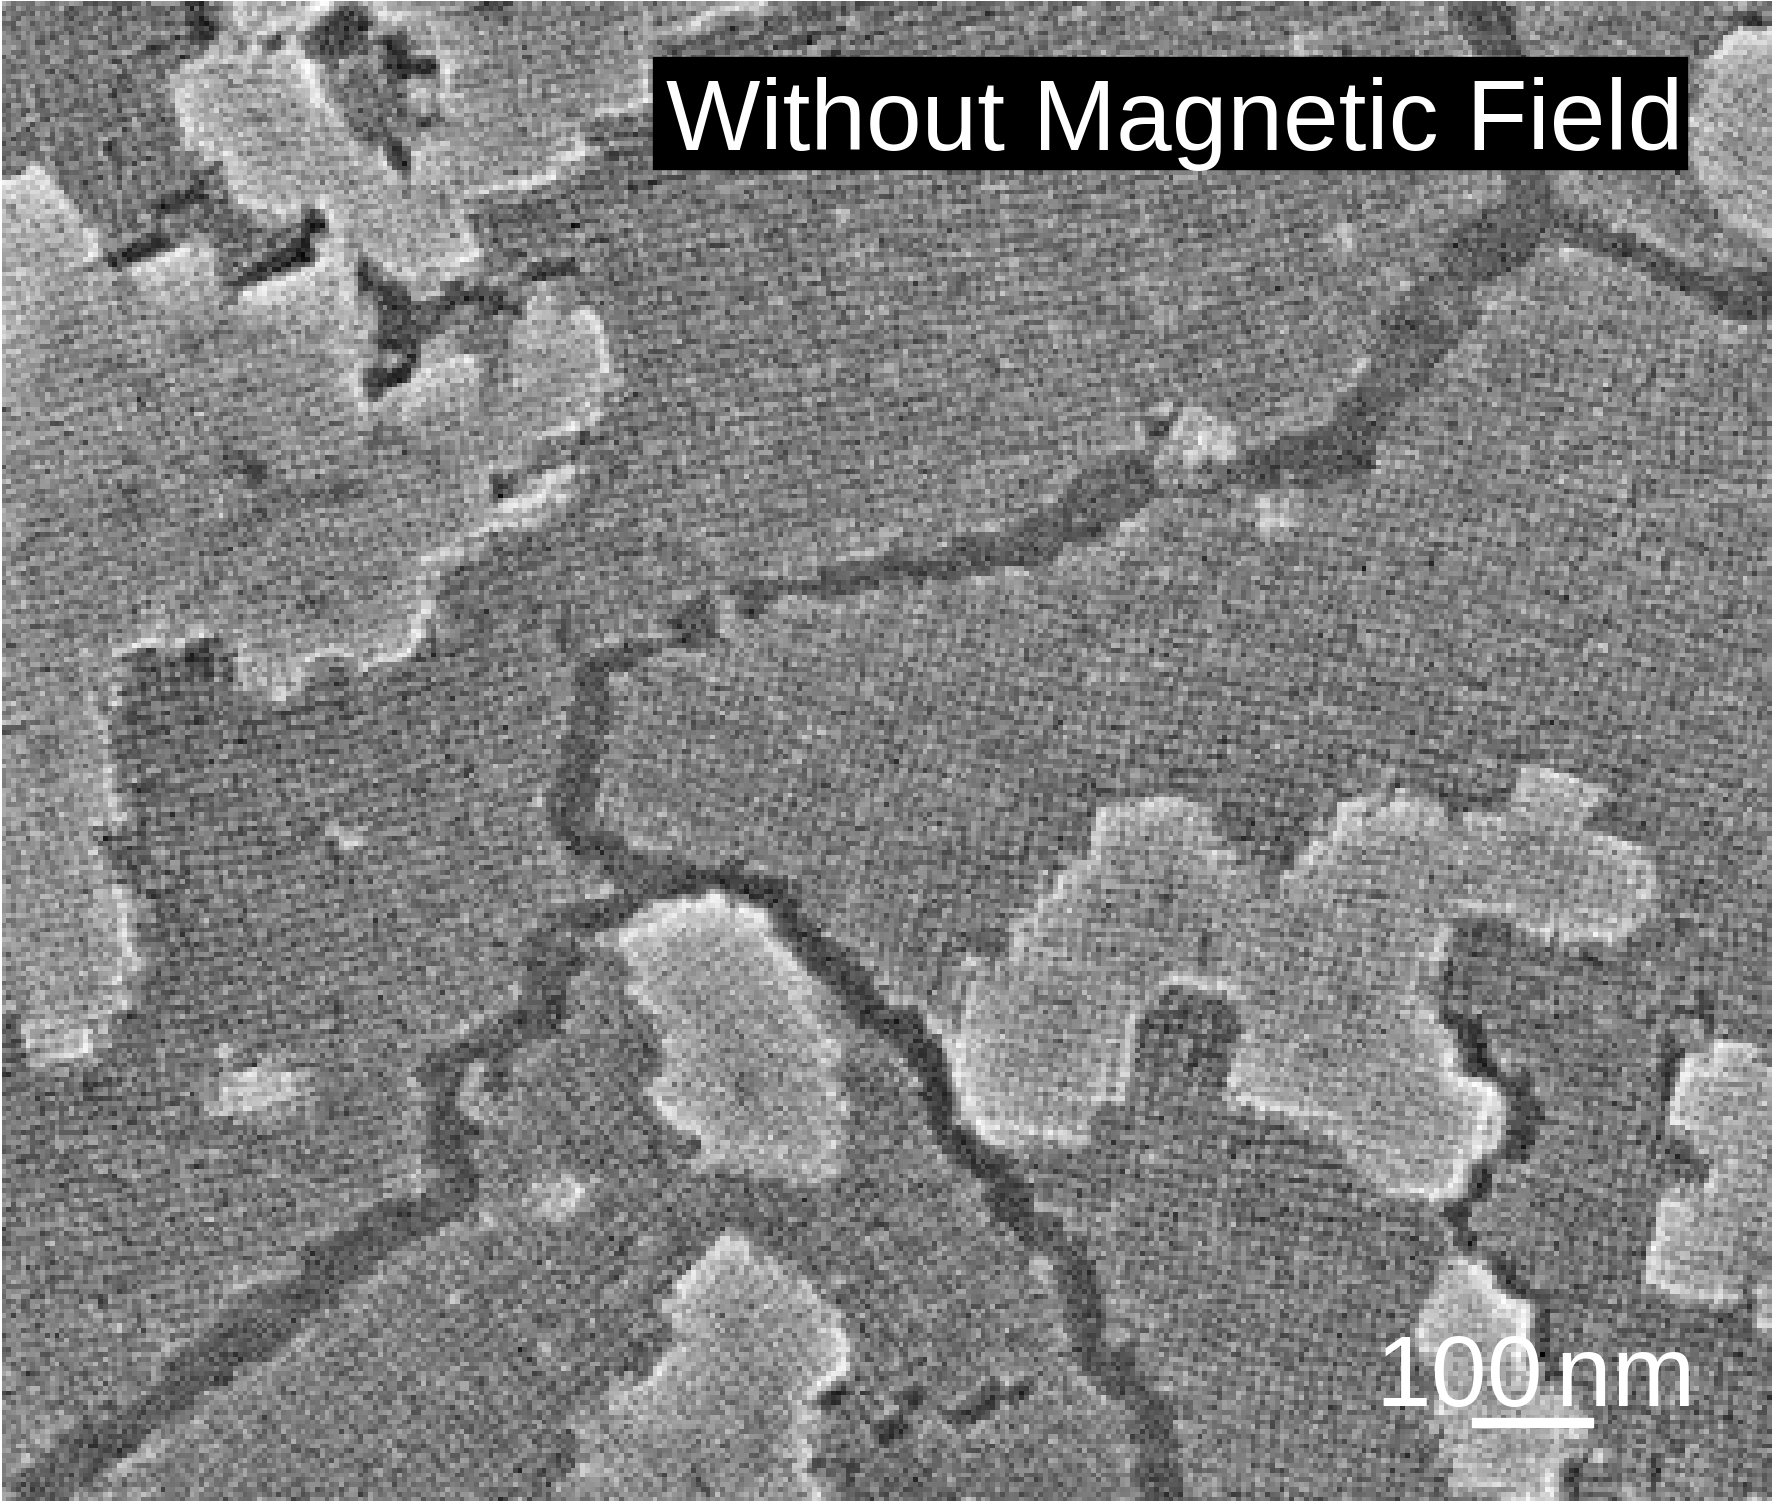
\includegraphics{monolayers_SEM_without_mag_field}
      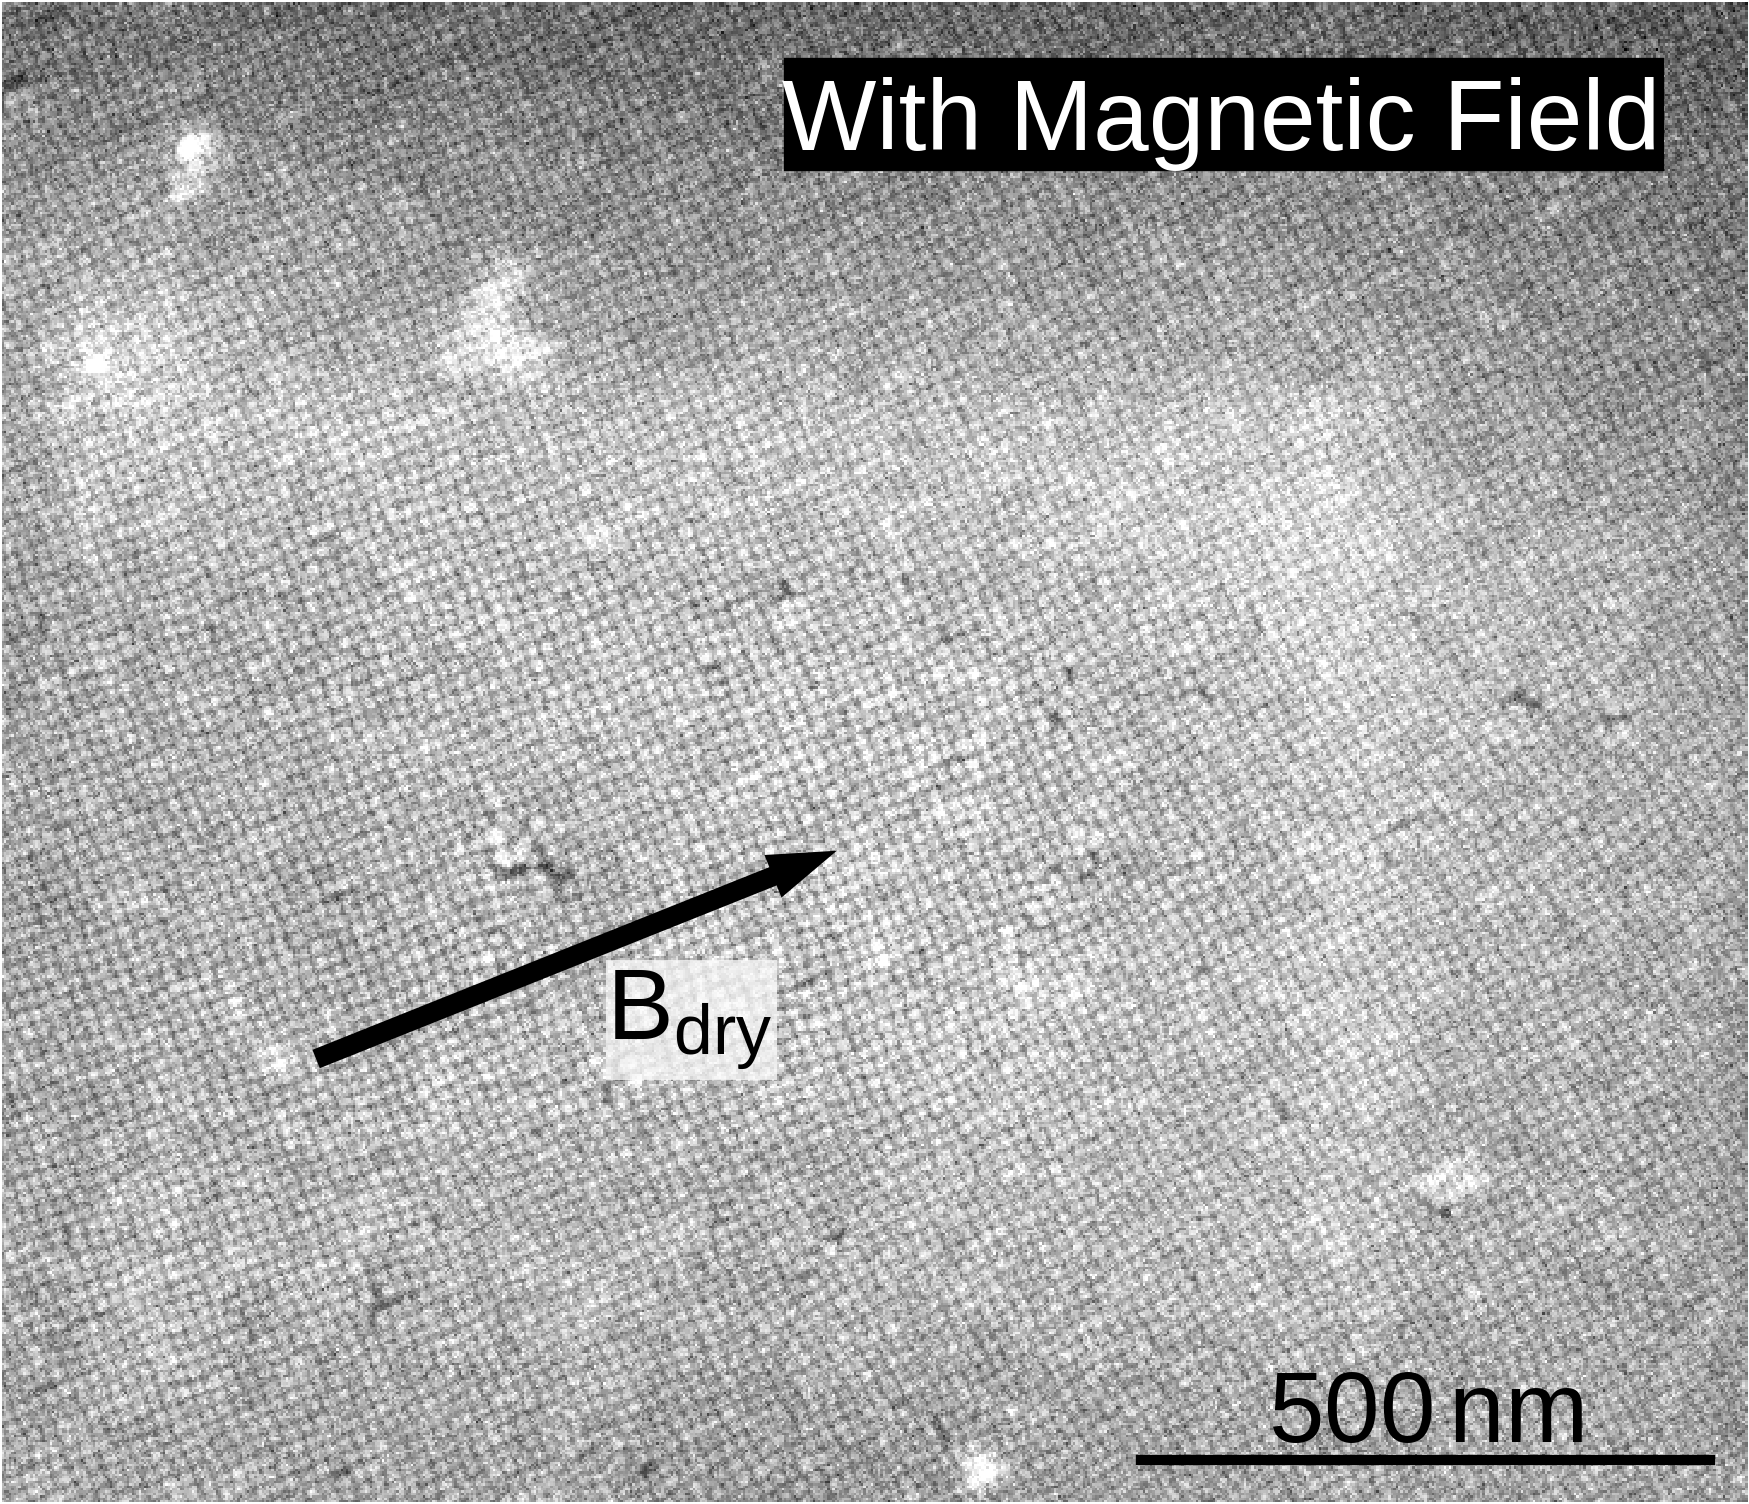
\includegraphics{monolayers_SEM_with_mag_field}
      \caption{\label{fig:monolayers:preparation:dryingConditions:magneticField}Comparison of simultaneously prepared monolayer from the same dispersion, one without applying a magnetic field, one within a Halbach cylinder with $B_{dry} \eq 40 \unit{mT}$.}
    \end{figure}
    Applying an in-plane magnetic field to strongly magnetic nanocubes during the first drying stages by the means of an Halbach cylinder, shown in the right image of \reffig{fig:monolayers:preparation:dryingConditions:varyConditions}, shows qualitatively a reduction of lattice defects and a tendency of aligning the cubes with the (100) faces along the magnetic field, which is visible in the SEM micrographs shown in \reffig{fig:monolayers:preparation:dryingConditions:magneticField}.
    Without a magnetic field, the sample consists of multiple large long-range ordered sheets, which are randomly oriented, which is no longer the case for the sample dried in magnetic field.
    A detailed quantitative study of oriented monolayer structures is, however, not in the scope of this thesis and left for future studies.

  \subsubsection{Second Stage: Slow Evaporating Components}
    \begin{figure}[tb]
      \centering
      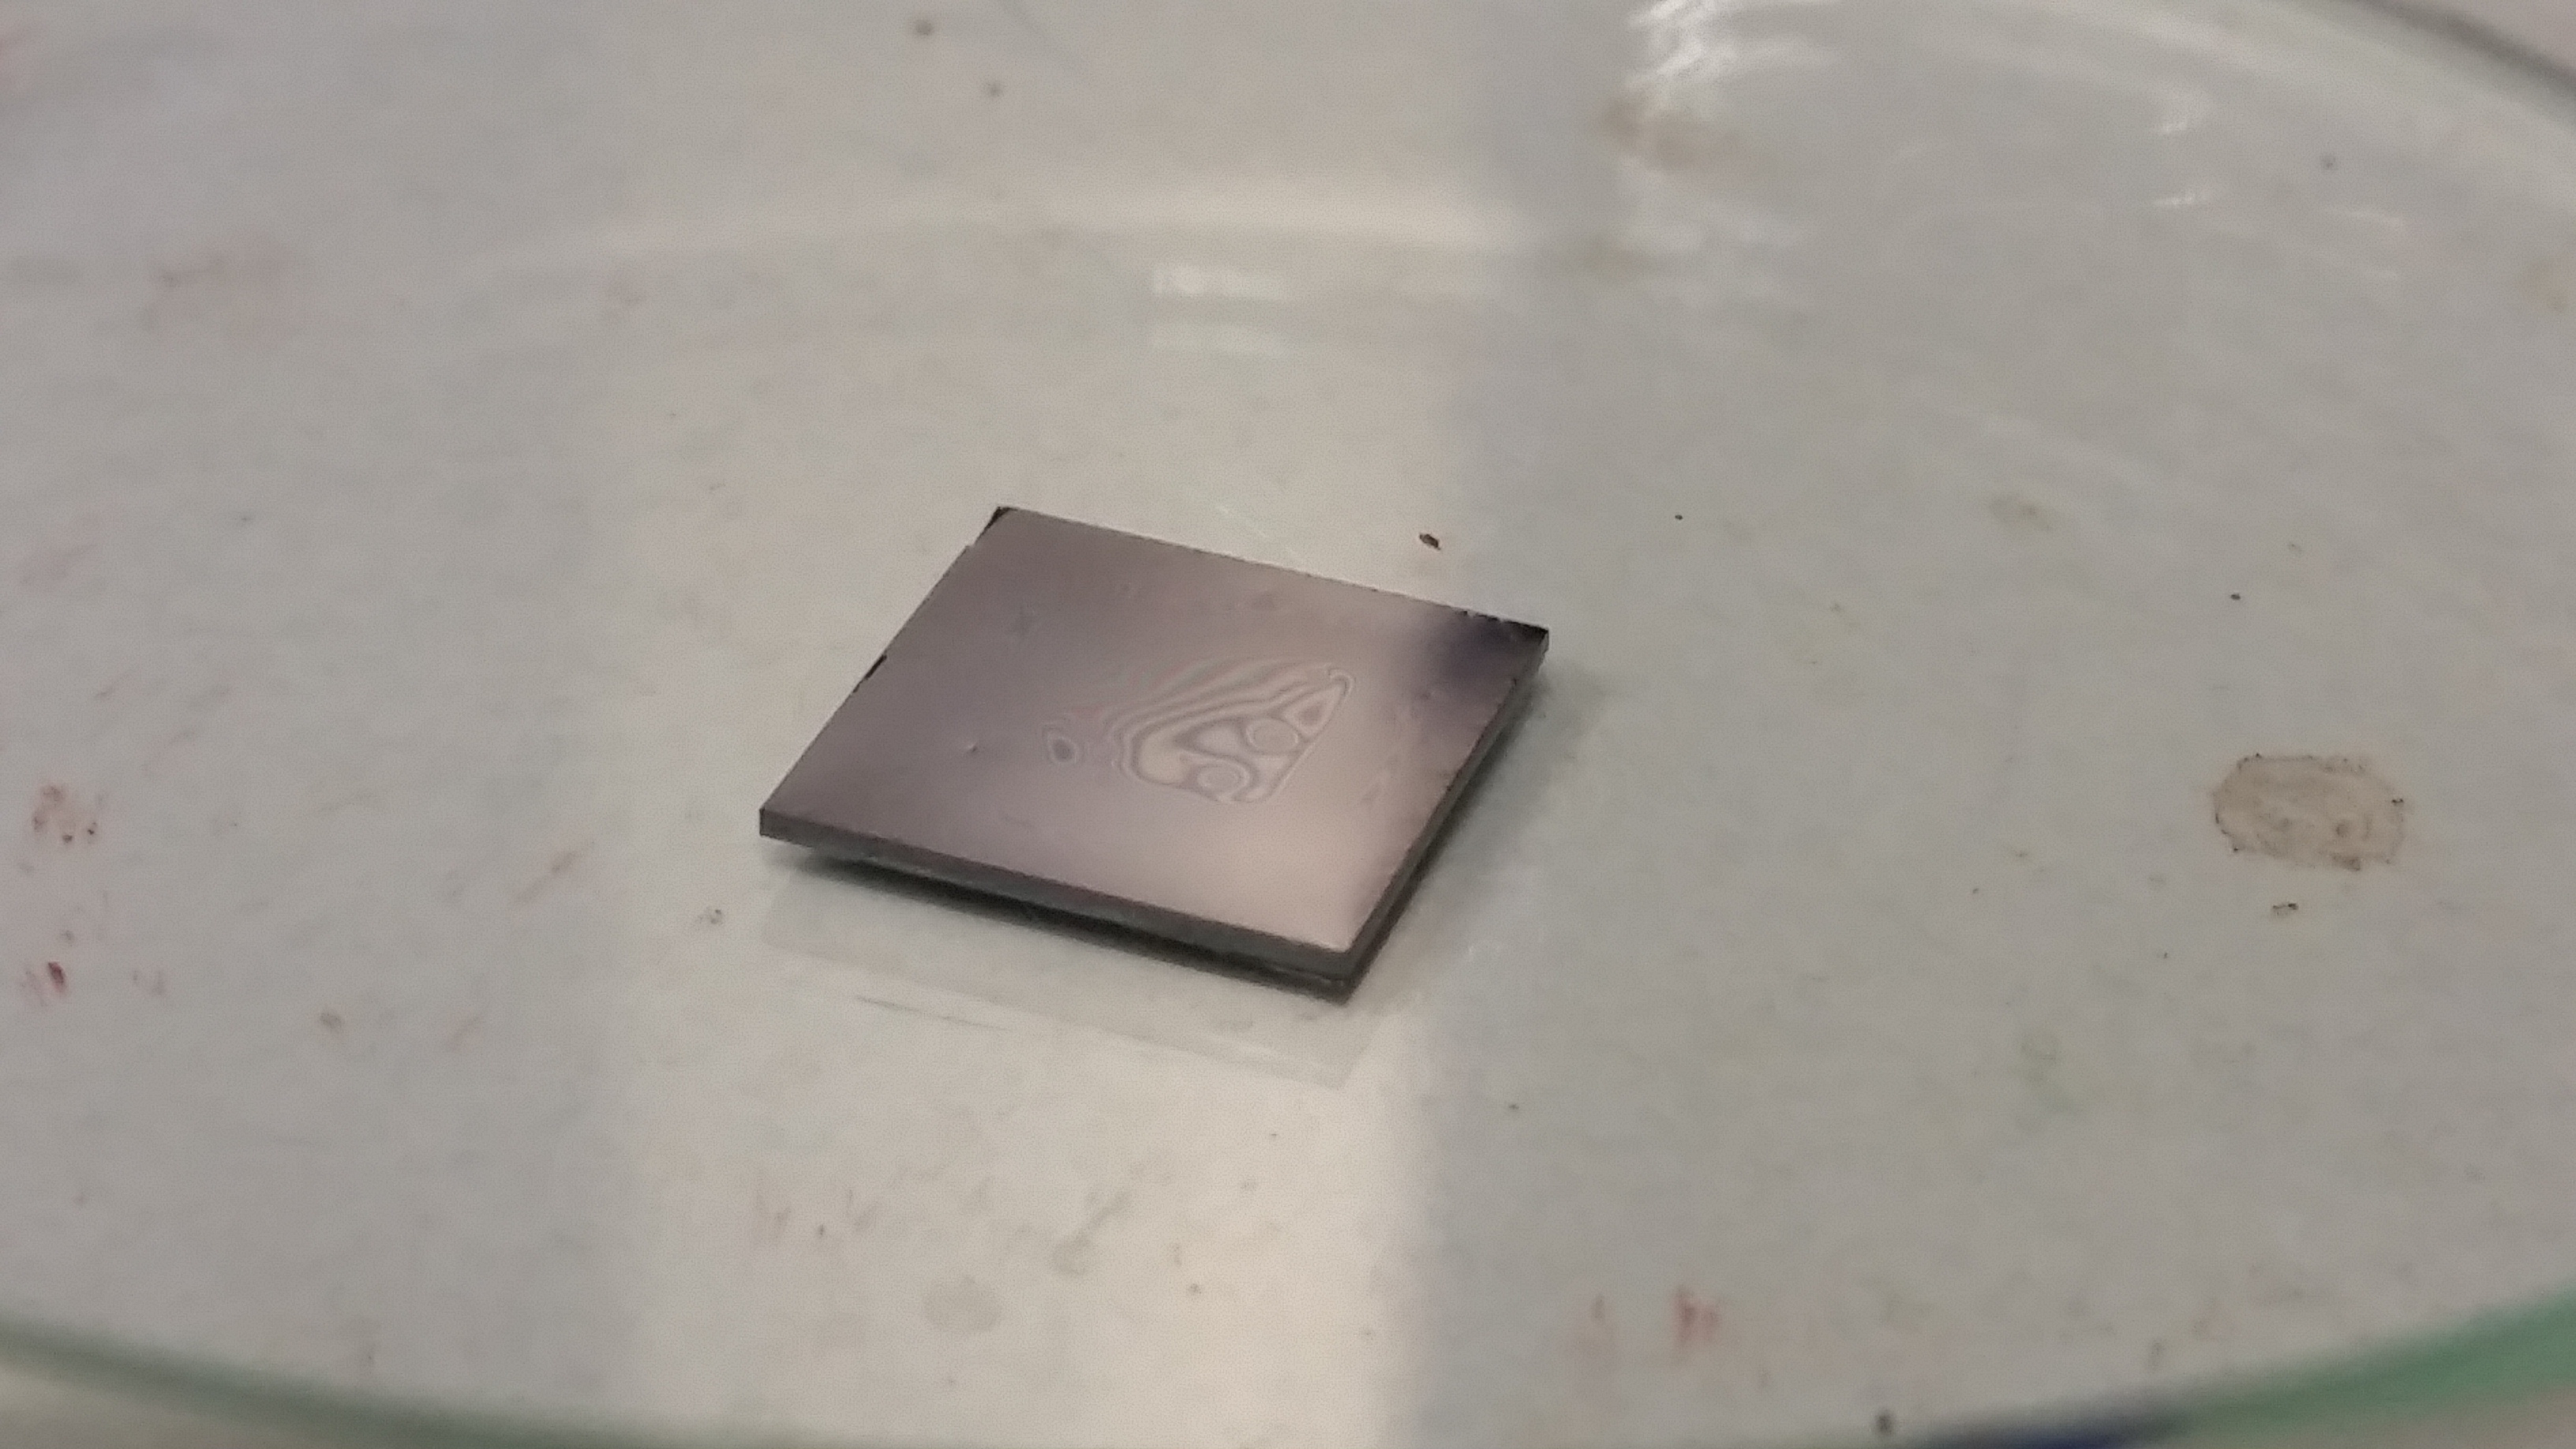
\includegraphics[width=0.7\textwidth]{monolayers_preparation_oilyFilm}
      \caption{\label{fig:monolayers:preparation:dryingConditions:oilyFilm}Thin oily film visible on a silicon wafer after the fast evaporating component of the dispersion has been dried during monolayer preparation.}
    \end{figure}

    After the fast evaporating component of the dispersion is dry, a thin oily film is visible on the wafer by thin-film interference, shown in \reffig{fig:monolayers:preparation:dryingConditions:oilyFilm}.
    Leaving the oily film on the substrate to rest for several weeks shows no sign of evaporation of the thin-film.
    Increasing the temperature of the wafer by a heating plate, speeds up the drying of the oily film but produces an inhomogeneous drying pattern that is visible by eye.
    The slow baking in an oven after the evaporation of the primary solvent at relatively low temperatures has proven to be the best method to produce a homogeneous evaporation of the secondary phase.
    By successively increasing the temperature of an oven, it was found that a temperature of approximately $140 \unit{^\circ C}$ is necessary to be applied to the monolayer for at least $6 \unit{h}$ to remove the organic compounds to most parts in the time frame of $1 - 2 \unit{days}$.

    To have a homogeneous evaporation, the best found method is to place the substrate within a glass Petri dish that is covered with an aluminum foil, which is perforated along the edge.
    The aluminum foil protects the wafer for one from dust and from other dirt in the oven, while it also directs the evaporating flow to controllably stream out the perforated edge.
    The temperature of the oven has been varied and the best result was observed for a two-step heating when the thin film of 1-octadecene/oleic acid is left within the oven at $80 \unit{^\circ C}$ for at least $12\unit{h}$ and then heated to $140 \unit{^\circ C}$ for at least $6\unit{h}$.

    An important technical observation that has to be considered is that the oven needs to be properly balanced with a water level.
    Any slope of just a few degrees leads to an accumulation at one side of the substrate as the gravitational force pulls the thin film to one side.
    When those steps are all considered, the second drying step leads to a homogeneous drying of most parts of the 1-octadecene/oleic acid.
    After the heating process, there is however often still some remaining organic components on the wafer surface that cannot be removed at $140 \unit{^\circ C}$, even when the sample is left for a week in the oven.
    One option is to increase the temperature even higher and be more aggressive in the evaporation of the organic solvents.
    However, attempts in that direction also result in a partial destruction of the long range order of the nanostructure.
    Therefore, the remaining organic layer is either accepted in the studied samples of this work or the prepared samples are washed.

    The idea here is to wash the prepared with a polar solvent, such as ethyl acetate.
    The polar solvents leave the long-range order unaffected, as the nanoparticles are only disperseable in non-polar solvents and the individual nanoparticles are stabilized by the nanostructure to remain on the substrate.
    The additional organic solvent, even though it is also not disperseable in polar solvents, can be removed this way by removing the polar solvent with the use of a spin coater.
    The loose organic solvents are detached by the polar solvent and carried off due to centrifugal force (note here that the density of ethyl acetate is slightly below the density of oleic acid).
    As ethyl acetate might also leave some organic remains, the sample is further washed again afterwards with 2-propanol (HPLC) to increase the cleanness of the nanoparticle surface from any unwanted organic remnants.
\end{document}